\documentclass[12pt, a4paper]{article}
\usepackage[utf8]{inputenc}
\usepackage[T5]{fontenc}
\usepackage[vietnamese]{babel}
\usepackage[a4paper, left=3cm, right=2cm, top=2.5cm, bottom=2.5cm]{geometry}
\usepackage{amsmath, amssymb, amsfonts}
\usepackage{booktabs}
\usepackage{array}
\usepackage{float}
\usepackage{multirow}
\usepackage{graphicx}
\usepackage{hyperref}
\usepackage{listings}
\usepackage{xcolor}

\hypersetup{
    colorlinks=true,
    linkcolor=blue,
    filecolor=magenta,      
    urlcolor=cyan,
    pdftitle={Báo cáo môn học HVAC XGB-DQN},
    pdfpagemode=FullScreen,
}

% Định nghĩa màu sắc cho code listings
\definecolor{codegreen}{rgb}{0,0.6,0}
\definecolor{codegray}{rgb}{0.5,0.5,0.5}
\definecolor{codepurple}{rgb}{0.58,0,0.82}
\definecolor{backcolour}{rgb}{0.95,0.95,0.92}

\lstdefinestyle{mystyle}{
    backgroundcolor=\color{backcolour},   
    commentstyle=\color{codegreen},
    keywordstyle=\color{magenta},
    numberstyle=\tiny\color{codegray},
    stringstyle=\color{codepurple},
    basicstyle=\ttfamily\footnotesize,
    breakatwhitespace=false,         
    breaklines=true,                 
    captionpos=b,                    
    keepspaces=true,                 
    numbers=left,                    
    numbersep=5pt,                  
    showspaces=false,                
    showstringspaces=false,
    showtabs=false,                  
    tabsize=2
}
\lstset{style=mystyle}

\begin{document}

% --- TRANG BÌA ---
\begin{titlepage}
    \begin{center}
        \textbf{\large TRƯỜNG ĐẠI HỌC BÁCH KHOA HÀ NỘI} \\
        \textbf{\large VIỆN CÔNG NGHỆ THÔNG TIN VÀ TRUYỀN THÔNG} \\
        \vskip 1.5cm
        
\includegraphics[width=0.18\textwidth]{hust_logo.png} % Dự phòng nếu có logo
        \vskip 1.5cm
        \textbf{\Large BÁO CÁO BÀI TẬP LỚN MÔN HỌC} \\
        \vskip 0.5cm
        \textbf{\huge HỌC MÁY VÀ ỨNG DỤNG} \\
        \vskip 1.5cm
        \noindent\rule{\textwidth}{1pt} \\
        \vskip 0.5cm
        \textbf{\Large ĐỀ TÀI: MÔ HÌNH LAI XGB-DQN ĐIỀU KHIỂN HỆ THỐNG HVAC VÀ CỬA SỔ TỰ ĐỘNG TỐI ƯU HÓA NĂNG LƯỢNG VÀ TIỆN NGHI NHIỆT} \\
        \vskip 0.5cm
        \noindent\rule{\textwidth}{1pt} \\
        \vskip 2cm
        \begin{flushright}
            \begin{tabular}{ll}
                \textbf{Giảng viên hướng dẫn:} & [Tên Giảng Viên] \\
                \textbf{Nhóm thực hiện:} & Nhóm 3 thành viên \\
                \textbf{Thành viên nhóm:} & 1. [Tên Thành Viên 1] - [MSSV 1] \\
                 & 2. [Tên Thành Viên 2] - [MSSV 2] \\
                 & 3. [Tên Thành Viên 3] - [MSSV 3] \\
                \textbf{Lớp:} & [Tên Lớp Học]
            \end{tabular}
        \end{flushright}
        \vfill
        \textbf{Hà Nội, Tháng 6 Năm 2026}
    \end{center}
\end{titlepage}

\newpage
\tableofcontents
\newpage

% --- NỘI DUNG ---
\section{Mở đầu}
Hệ thống Sưởi, Thông gió và Điều hòa không khí (HVAC) đóng vai trò quyết định trong việc duy trì chất lượng không khí và tiện nghi nhiệt trong các công trình kiến trúc hiện đại. Theo báo cáo của Ủy ban Liên chính phủ về Biến đổi Khí hậu (IPCC) và các thống kê năng lượng toàn cầu, vận hành tòa nhà chiếm khoảng 40\% tổng năng lượng tiêu thụ sơ cấp, trong đó hơn 50\% điện năng của các tòa nhà thương mại và dân cư được dùng để chạy hệ thống điều hòa không khí. Tại Việt Nam, một quốc gia thuộc vùng khí hậu nhiệt đới gió mùa nóng ẩm, nhu cầu làm mát vào mùa hè tại các đô thị lớn như Hà Nội và Thành phố Hồ Chí Minh là vô cùng lớn, gây áp lực nặng nề lên hệ thống lưới điện quốc gia. Do đó, việc tìm kiếm các giải pháp điều khiển HVAC tối ưu là một yêu cầu vô cùng cấp bách nhằm dung hòa giữa bài toán tiết kiệm năng lượng và đảm bảo năng suất làm việc, sức khỏe của con người thông qua sự thoải mái nhiệt.

Các phương pháp điều khiển HVAC truyền thống, chẳng hạn như bộ điều khiển Rule-based (RBC) dựa trên các ngưỡng cố định hoặc các bộ điều khiển dựa trên lịch trình tĩnh, bộc lộ nhiều hạn chế nghiêm trọng. Chúng không có khả năng thích ứng linh hoạt trước sự thay đổi liên tục của thời tiết bên ngoài, quán tính nhiệt lớn và có tính phi tuyến cao của tòa nhà, cũng như sự thay đổi ngẫu nhiên của mật độ người sử dụng (occupancy profile). Điều này dẫn đến tình trạng làm lạnh quá mức gây lãng phí năng lượng nghiêm trọng, hoặc không đảm bảo đủ điều kiện tiện nghi cho con người.

Để giải quyết bài toán tối ưu hóa đa mục tiêu phức tạp này, các nghiên cứu gần đây đã hướng tới việc áp dụng Học tăng cường (Reinforcement Learning - RL) để tự động hóa quá trình ra quyết định. Việc kết hợp điều khiển hành vi của con người (Occupant-centric Control - OCC) và phối hợp trạng thái đóng/mở cửa sổ tự nhiên cùng điều hòa mang lại tiềm năng tiết kiệm năng lượng vượt trội. Đề tài này tập trung vào việc nghiên cứu, tái hiện và cải tiến mô hình lai XGB-DQN được đề xuất bởi nhóm nghiên cứu WHU-LX trong bài báo \textit{"Occupant-centric HVAC and window control: A reinforcement learning model for enhancing indoor thermal comfort and energy efficiency"}. 

Báo cáo này được cấu trúc như sau:
\begin{itemize}
    \item \textbf{Mục 2} giới thiệu chi tiết cơ sở lý thuyết toán học của mô hình lai XGB-DQN, bao gồm mô hình Surrogate XGBoost và thuật toán DQN điều khiển.
    \item \textbf{Mục 3} phân tích chuyên sâu các lỗi logic và hạn chế kỹ thuật nghiêm trọng trong mã nguồn của repo gốc WHU-LX dẫn đến việc tác tử bị overfit và hoàn toàn tắt điều hòa (0\% AC).
    \item \textbf{Mục 4} trình bày chi tiết 4 giải pháp cải tiến thuật toán của nhóm đề xuất để khắc phục triệt để các lỗi này.
    \item \textbf{Mục 5} phân tích sâu kết quả thực nghiệm đạt được trên mô hình Surrogate XGBoost và giải nghĩa định lượng các đồ thị kết quả.
    \item \textbf{Mục 6} trình bày kết quả kiểm chứng nâng cao của tác tử trên môi trường mô phỏng động học vật lý thực tế Sinergym + EnergyPlus cho khí hậu Thành phố Hồ Chí Minh.
    \item \textbf{Mục 7} đưa ra các kết luận tổng kết và định hướng nghiên cứu tiếp theo.
\end{itemize}

\section{Cơ sở lý thuyết của hệ thống XGB-DQN}
Hệ thống điều khiển phối hợp HVAC và cửa sổ tự động lai bao gồm hai thành phần hoạt động phối hợp chặt chẽ: mô hình học máy XGBoost đóng vai trò giả lập môi trường nhiệt tòa nhà (Surrogate Model) và mạng DQN đóng vai trò tác tử học tăng cường ra quyết định điều khiển (Control Agent).

\subsection{Mô hình môi trường gần đúng XGBoost (Surrogate Model)}
Huấn luyện trực tiếp một tác tử RL trên các hệ thống thực tế hoặc qua các phần mềm mô phỏng vật lý như EnergyPlus rất tốn thời gian (thường mất từ vài giờ đến vài ngày cho một đợt chạy). Để tăng tốc độ huấn luyện, mô hình Surrogate được sử dụng. XGBoost (Extreme Gradient Boosting), một thuật toán học máy mạnh mẽ dựa trên cây quyết định nâng cao (Gradient Boosted Decision Trees - GBDT), được huấn luyện trên dữ liệu lịch sử để học động học nhiệt của phòng.

Mô hình XGBoost học hàm ánh xạ $f_{XGB}$ để dự đoán độ lệch nhiệt độ phòng giữa thời điểm $t+1$ và $t$:
\begin{equation}
\Delta T_{in}(t) = T_{in}(t+1) - T_{in}(t) = f_{XGB}(s_t, a_t)
\end{equation}

Mục tiêu huấn luyện của XGBoost tại mỗi cây thứ $k$ là tối thiểu hóa hàm mục tiêu có chứa thành phần phạt chính quy hóa để chống overfitting:
\begin{equation}
\mathcal{L}^{(k)} = \sum_{i=1}^{N} l\left(y_i, \hat{y}_i^{(k-1)} + f_k(x_i)\right) + \Omega(f_k)
\end{equation}
Trong đó, $\Omega(f_k) = \gamma T_k + \frac{1}{2} \lambda \sum_{j=1}^{T_k} w_j^2$ là thành phần phạt dựa trên số lượng lá $T_k$ và trọng số của các lá $w_j$ của cây thứ $k$. Hàm loss $l$ được xấp xỉ bậc hai bằng khai triển Taylor:
\begin{equation}
\mathcal{L}^{(k)} \approx \sum_{i=1}^{N} \left[ l(y_i, \hat{y}_i^{(k-1)}) + g_i f_k(x_i) + \frac{1}{2} h_i f_k^2(x_i) \right] + \gamma T_k + \frac{1}{2} \lambda \sum_{j=1}^{T_k} w_j^2
\end{equation}
Với $g_i$ và $h_i$ lần lượt là đạo hàm bậc nhất (gradient) và bậc hai (hessian) của hàm loss đối với giá trị dự đoán ở bước trước đó.

Trạng thái môi trường $s_t$ bao gồm 8 biến trạng thái phòng và thời tiết tại thời điểm $t$:
\begin{equation}
s_t = [T_{in}(t), RH_{in}(t), T_{out}(t), RH_{out}(t), R(t), C(t), W_s(t), H(t)]
\end{equation}
Trong đó:
\begin{itemize}
    \item $T_{in}(t), RH_{in}(t)$: Nhiệt độ ($^\circ\text{C}$) và độ ẩm tương đối (\%) trong phòng.
    \item $T_{out}(t), RH_{out}(t)$: Nhiệt độ ($^\circ\text{C}$) và độ ẩm tương đối (\%) ngoài trời.
    \item $R(t), C(t), W_s(t)$: Lượng mưa, độ che phủ mây và tốc độ gió ngoài trời.
    \item $H(t)$: Giờ trong ngày (0 - 23).
\end{itemize}
Hành động $a_t$ đại diện cho thiết lập điều khiển tại bước thời gian $t$. Nhiệt độ phòng ở bước tiếp theo được cập nhật bằng công thức:
\begin{equation}
T_{in}(t+1) = T_{in}(t) + \Delta T_{in}(t)
\end{equation}

\subsection{Tác tử Học tăng cường Q-Learning sâu (DQN)}
Nhiệm vụ điều khiển được phát biểu dưới dạng một bài toán Quyết định Markov (Markov Decision Process - MDP) với không gian trạng thái $S$, không gian hành động $A$, hàm chuyển trạng thái và hàm nhận thưởng $R$. Do không gian trạng thái $S$ chứa các biến liên tục có kích thước lớn, việc áp dụng bảng Q-table thông thường sẽ dẫn tới hiện tượng bùng nổ chiều (curse of dimensionality). Do đó, DQN sử dụng một mạng thần kinh đa lớp (MLP) làm bộ xấp xỉ hàm trị số $Q(s, a; \theta)$ nhằm dự đoán giá trị Q-value cho từng hành động.

\subsubsection{Không gian hành động (Action Space)}
Tác tử điều khiển phối hợp cả thiết lập nhiệt độ làm lạnh của điều hòa không khí (AC cooling setpoint) và trạng thái đóng/mở cửa sổ. Không gian hành động bao gồm 24 hành động rời rạc ($A \in \{0, 1, ..., 23\}$) được định nghĩa chi tiết trong Bảng \ref{tab:action_definitions}.

\begin{table}[H]
    \centering
    \caption{Định nghĩa chi tiết 24 hành động trong không gian hành động của tác tử}
    \label{tab:action_definitions}
    \vspace{0.2cm}
    \begin{tabular}{cccc}
        \toprule
        \textbf{Chỉ số hành động} & \textbf{Trạng thái AC} & \textbf{Setpoint AC ($^\circ\text{C}$)} & \textbf{Trạng thái Cửa sổ} \\
        \midrule
        0 & Tắt & - & Đóng \\
        1 - 11 & Bật & $19 + a$ (tức là $20^\circ\text{C} - 30^\circ\text{C}$) & Đóng \\
        12 & Tắt & - & Mở \\
        13 - 23 & Bật & $a + 7$ (tức là $20^\circ\text{C} - 30^\circ\text{C}$) & Mở \\
        \bottomrule
    \end{tabular}
\end{table}

\subsubsection{Hàm Reward và Tiêu chuẩn Tiện nghi Nhiệt Thích ứng ASHRAE 55}
Hàm reward của tác tử được thiết kế nhằm dung hòa hai mục tiêu đối nghịch: duy trì tiện nghi nhiệt và tiết kiệm năng lượng tiêu thụ:
\begin{equation}
R(s, a, s') = w_c \cdot P_{comfort}(s') + P_{energy}(a)
\end{equation}
Trong đó, $w_c$ là trọng số điều chỉnh mức độ ưu tiên của tiện nghi nhiệt. 

Mức phạt tiện nghi $P_{comfort}(s')$ được xác định dựa trên lý thuyết tiện nghi thích ứng (Adaptive Comfort Model) của tiêu chuẩn \textbf{ASHRAE Standard 55}. Dải nhiệt độ dễ chịu của phòng $[L_c, U_c]$ phụ thuộc tuyến tính vào nhiệt độ trung bình ngoài trời $T_{out}$. Thuật toán xác định dải giới hạn theo công thức nội suy tuyến tính từng đoạn:
\begin{itemize}
    \item Nếu $T_{out} \le 10^\circ\text{C}$:
    \begin{equation}
    L_c = 18.4^\circ\text{C}, \quad U_c = 23.4^\circ\text{C}
    \end{equation}
    \item Nếu $T_{out} \ge 30^\circ\text{C}$:
    \begin{equation}
    L_c = 24.6^\circ\text{C}, \quad U_c = 29.6^\circ\text{C}
    \end{equation}
    \item Nếu $10^\circ\text{C} < T_{out} < 30^\circ\text{C}$:
    \begin{equation}
    L_c(T_{out}) = 18.4 + \frac{T_{out} - 10}{20} \times (24.6 - 18.4)
    \end{equation}
    \begin{equation}
    U_c(T_{out}) = 23.4 + \frac{T_{out} - 10}{20} \times (29.6 - 23.4)
    \end{equation}
\end{itemize}

Hình phạt tiện nghi được tính bằng bình phương khoảng cách lệch nhiệt độ khi phòng nằm ngoài dải thoải mái thích ứng:
\begin{equation}
P_{comfort}(s') = \begin{cases}
0 & \text{nếu } L_c \le T_{in}' \le U_c \\
-(T_{in}' - L_c)^2 & \text{nếu } T_{in}' < L_c \\
-(T_{in}' - U_c)^2 & \text{nếu } T_{in}' > U_c
\end{cases}
\end{equation}
Hình phạt năng lượng $P_{energy}(a)$ phản ánh công suất điện tiêu thụ tương đương của các thiết lập điều khiển (giá trị phạt dựa trên đặc tính công suất điện năng tương đương của hệ thống điều hòa):
\begin{equation}
P_{energy}(a) = \begin{cases}
0 & \text{nếu } a \in \{0, 12\} \text{ (AC tắt)} \\
-(60 \times 0.87 \times 1) = -52.2 & \text{nếu } 0 < a < 12 \text{ (AC bật, cửa sổ đóng)} \\
-2 \times (60 \times 0.87 \times 1) = -104.4 & \text{nếu } a > 12 \text{ (AC bật, cửa sổ mở - phạt gấp đôi)}
\end{cases}
\end{equation}

\subsubsection{Cập nhật Mạng Thần kinh DQN}
Tác tử sử dụng một mạng thần kinh đa lớp (MLP) làm bộ xấp xỉ hàm trị số $Q(s, a; \theta)$. Để huấn luyện mạng, tác tử lấy mẫu ngẫu nhiên một batch trải nghiệm $(s, a, s', r)$ từ Bộ nhớ đệm trải nghiệm (Replay Buffer) $\mathcal{D}$ có dung lượng cố định nhằm phá vỡ tính tương quan thời gian của dữ liệu huấn luyện. Trọng số $\theta$ được cập nhật bằng cách cực tiểu hóa hàm Loss bình phương sai số TD (Temporal Difference):
\begin{equation}
L(\theta) = \frac{1}{B} \sum_{i=1}^{B} \left( y_i - Q(s_i, a_i; \theta) \right)^2
\end{equation}
Trong đó, $B$ là kích thước batch, và mục tiêu TD $y_i$ được tính bằng mạng Target Network có trọng số $\theta^-$ để tránh hiện tượng dịch chuyển mục tiêu liên tục gây mất ổn định:
\begin{equation}
y_i = r_i + \gamma \max_{a'} Q(s_i', a'; \theta^-)
\end{equation}

\section{Phân tích hạn chế kỹ thuật của repo gốc WHU-LX}
Qua khảo sát và kiểm thử trực tiếp mã nguồn gốc của WHU-LX, nhóm nghiên cứu đã phát hiện ra các lỗi thiết kế thuật toán vô cùng nghiêm trọng. Đây là nguyên nhân cốt lõi khiến tác nhân DQN gốc đạt hiệu năng kém và không có khả năng vận hành thực tế.

\subsection{Lỗi Quá khớp Đơn ngày (Single-day Overfitting)}
Trong mã nguồn huấn luyện gốc, tác giả cố định tham số dữ liệu đầu vào chỉ chạy trên đúng ngày đầu tiên của bộ dữ liệu (\texttt{day\_index = 0}). Vòng lặp huấn luyện DQN chạy qua 1.000 episodes nhưng chỉ lặp đi lặp lại việc mô phỏng 12 giờ làm việc của đúng ngày này. 
Do ngày \texttt{day\_index = 0} có điều kiện thời tiết vô cùng mát mẻ (chuyển mùa), tác tử nhanh chóng học được rằng chỉ cần mở cửa sổ ($a = 12$) hoặc tắt điều hòa, đóng cửa ($a = 0$) là nhiệt độ phòng tự động nằm trong dải tiện nghi. DQN bị quá khớp cực đoan vào kiểu thời tiết này và rút ra kết luận sai lầm: không cần bật AC trong mọi trường hợp.

\subsection{Sự bất đối xứng về biên độ trong hàm phạt Reward (Lỗi 0\% AC)}
Hàm phạt reward nguyên bản được cấu hình với trọng số tiện nghi mặc định $w_c = 1.0$. Chúng ta hãy cùng thực hiện một phân tích định lượng chi tiết để làm rõ lý do tại sao mạng DQN gốc hoàn toàn tê liệt khả năng bật AC:
\begin{itemize}
    \item Giả sử nhiệt độ phòng nóng lên tới $27.5^\circ\text{C}$ trong khi dải giới hạn trên tiện nghi là $U_c = 26^\circ\text{C}$. Độ lệch nhiệt độ là $\Delta T = +1.5^\circ\text{C}$.
    \item Hình phạt tiện nghi khi tắt điều hòa sẽ là:
    \begin{equation}
    P_{comfort} = -(1.5)^2 = -2.25 \text{ điểm}
    \end{equation}
    \item Nếu tác tử chọn hành động bật điều hòa để làm mát phòng đưa nhiệt độ về dải tiện nghi ($\Delta T = 0$), nó sẽ chịu hình phạt tiêu thụ năng lượng cố định là:
    \begin{equation}
    P_{energy} = -52.2 \text{ điểm}
    \end{equation}
    \item So sánh điểm reward nhận được giữa hai quyết định:
    \begin{equation}
    R_{AC\_Off} = -2.25 > R_{AC\_On} = -52.2
    \end{equation}
\end{itemize}
Sự chênh lệch biên độ cực kỳ lớn (lên tới hơn 23 lần) khiến tác tử RL nhận thấy việc bật AC sẽ bị phạt cực kỳ nặng về mặt năng lượng, lớn hơn rất nhiều so với việc chấp nhận chịu nóng. Ngay cả khi phòng cực kỳ nóng ($31^\circ\text{C}$, lệch $5^\circ\text{C}$ thì phạt comfort cũng chỉ là $-25$ điểm, vẫn nhỏ hơn rất nhiều so với $-52.2$ điểm phạt AC). Mạng DQN đã tìm ra một cực trị địa phương lười biếng: \textbf{luôn luôn tắt điều hòa trong mọi tình huống (Tỷ lệ bật AC = 0.00\%)}. Khi đem đánh giá trên 1.763 ngày thời tiết quanh năm, tỷ lệ tiện nghi đạt được cực kỳ thấp (67.99\%).

\subsection{Thiếu cấu trúc mạng Target Network và Không chuẩn hóa State}
Mã nguồn gốc cập nhật giá trị Q trực tiếp bằng chính mạng đang huấn luyện (\texttt{target\_q\_values = q\_network(next\_states)}). Việc này vi phạm nguyên lý cơ bản của thuật toán DQN, khiến mục tiêu cập nhật thay đổi liên tục, gây mất ổn định nghiêm trọng trong quá trình tối ưu hóa. Đồng thời, trạng thái đầu vào chứa các biến có scale lệch nhau lớn (độ ẩm $\approx 80$, độ che phủ mây $\approx 0.1$, nhiệt độ $\approx 30$, giờ $\approx 23$) được feed trực tiếp vào mạng mà không chuẩn hóa, dẫn tới hiện tượng bão hòa gradient và làm tê liệt hoàn toàn khả năng học của các tầng Dense.

\section{Các cải tiến kỹ thuật đề xuất}
Nhóm nghiên cứu đã thực hiện sửa đổi triệt để cấu trúc mã nguồn trong file \texttt{reproduce\_whulx\_pipeline.py} bằng cách áp dụng 4 cải tiến thuật toán cốt lõi:

\begin{enumerate}
    \item \textbf{Huấn luyện Đa Ngày Ngẫu Nhiên (Multi-day Training):} Trong mỗi episode huấn luyện, tác tử sẽ lựa chọn ngẫu nhiên một ngày bất kỳ từ tập dữ liệu 1.763 ngày lịch sử để thực hiện rollout. Cách tiếp cận này giúp tác tử được tiếp xúc với toàn bộ phân phối thời tiết (nắng nóng mùa hè, mát mẻ mùa xuân, gió lạnh mùa đông), ép buộc DQN phải học cách tổng quát hóa hành vi điều khiển.
    \item \textbf{Tinh chỉnh Trọng số Reward (Reward Rescaling):} Nhóm đã thiết lập lại trọng số tiện nghi nhiệt $w_c = 120.0$. Lúc này, nếu phòng bị nóng lệch $1.5^\circ\text{C}$, hình phạt tiện nghi sẽ là $-1.5^2 \times 120 = -270.0$ điểm. Mức phạt này lớn hơn rất nhiều so với hình phạt năng lượng bật AC ($-52.2$). Nhờ đó, DQN có động lực mạnh mẽ để bật AC hạ nhiệt cứu tiện nghi, nhưng vẫn biết tắt AC khi phòng đã mát để tiết kiệm điện.
    \item \textbf{Tách biệt mạng Target Q-Network:} Khởi tạo mạng Target Network $\theta^-$ riêng biệt và cập nhật đồng bộ trọng số từ mạng chính $\theta$ định kỳ sau mỗi 10 episodes để đảm bảo tính ổn định toán học cho hàm mục tiêu TD.
    \item \textbf{Chuẩn hóa trạng thái Min-Max (State Normalization):} Toàn bộ vector trạng thái đầu vào được chuẩn hóa về dải $[0, 1]$ trước khi nạp vào mạng thần kinh để tối ưu hóa dòng truyền gradient:
    \begin{equation}
    T_{in, norm} = \frac{T_{in}}{40}, \quad RH_{norm} = \frac{RH}{100}, \quad T_{out, norm} = \frac{T_{out}}{40}, \quad H_{norm} = \frac{H}{23}
    \end{equation}
    Các biến Rain, Cloud, Windspeed cũng lần lượt được chia cho giá trị cực đại để đưa về dải chuẩn $[0, 1]$.
\end{enumerate}

Mạng DQN cải tiến được thiết kế dưới dạng MLP với 2 tầng ẩn (mỗi tầng chứa 64 unit kích hoạt bằng hàm ReLU), tốc độ học $\alpha = 0.001$, hệ số chiết khấu $\gamma = 0.95$. Chiến lược epsilon-greedy được áp dụng với mức epsilon giảm dần từ $1.0$ xuống $0.01$ để cân bằng khám phá và khai thác.

\section{Kết quả thực nghiệm trên mô hình Surrogate XGBoost}
Các thực nghiệm dưới đây được đánh giá trên toàn bộ tập dữ liệu 1.763 ngày lịch sử nhằm so sánh trực tiếp hiệu năng giữa tác nhân DQN cải tiến của nhóm, DQN gốc của WHU-LX và dữ liệu thực tế do con người vận hành (Human).

\subsection{Hiệu năng huấn luyện của XGBoost}
Mô hình Surrogate XGBoost đạt độ chính xác rất cao khi dự báo nhiệt độ phòng: Sai số tuyệt đối trung bình $\text{MAE} \approx 0.182^\circ\text{C}$, sai số căn phương trung bình $\text{RMSE} \approx 0.348^\circ\text{C}$, và hệ số tương quan xác định $\text{R}^2 \approx 0.48$. Điều này đảm bảo mô hình giả lập phản ánh trung thực động học nhiệt độ phòng để huấn luyện DQN.

\subsection{So sánh hiệu năng tổng thể trên tập đánh giá}
Bảng \ref{tab:comparison_focused} tóm tắt các chỉ số hiệu năng trung bình tích lũy thu được của ba đối tượng điều khiển trên toàn bộ tập dữ liệu.

\begin{table}[H]
    \centering
    \caption{Bảng so sánh hiệu năng các bộ điều khiển trên toàn bộ 1.763 ngày đánh giá}
    \label{tab:comparison_focused}
    \vspace{0.2cm}
    \begin{tabular}{lcccc}
        \toprule
        \textbf{Bộ điều khiển} & \textbf{Comfort (\%)} & \textbf{Tỉ lệ bật AC (\%)} & \textbf{Tỉ lệ mở cửa (\%)} & \textbf{Reward trung bình} \\
        \midrule
        \textbf{DQN Cải tiến (Nhóm)} & \textbf{78.55\%} & \textbf{66.97\%} & \textbf{30.93\%} & \textbf{-794.45} \\
        Human (Thực tế) & 72.84\% & 14.37\% & 52.17\% & \textit{N/A} \\
        DQN Gốc (WHU-LX) & 67.99\% & 0.00\% & 34.09\% & -14.51 \\
        \bottomrule
    \end{tabular}
\end{table}

\subsection{Phân tích chuyên sâu đồ thị kết quả}
Dưới đây là các phân tích chi tiết dựa trên các đồ thị kết quả huấn luyện và vận hành thu được:

\begin{figure}[H]
    \centering
    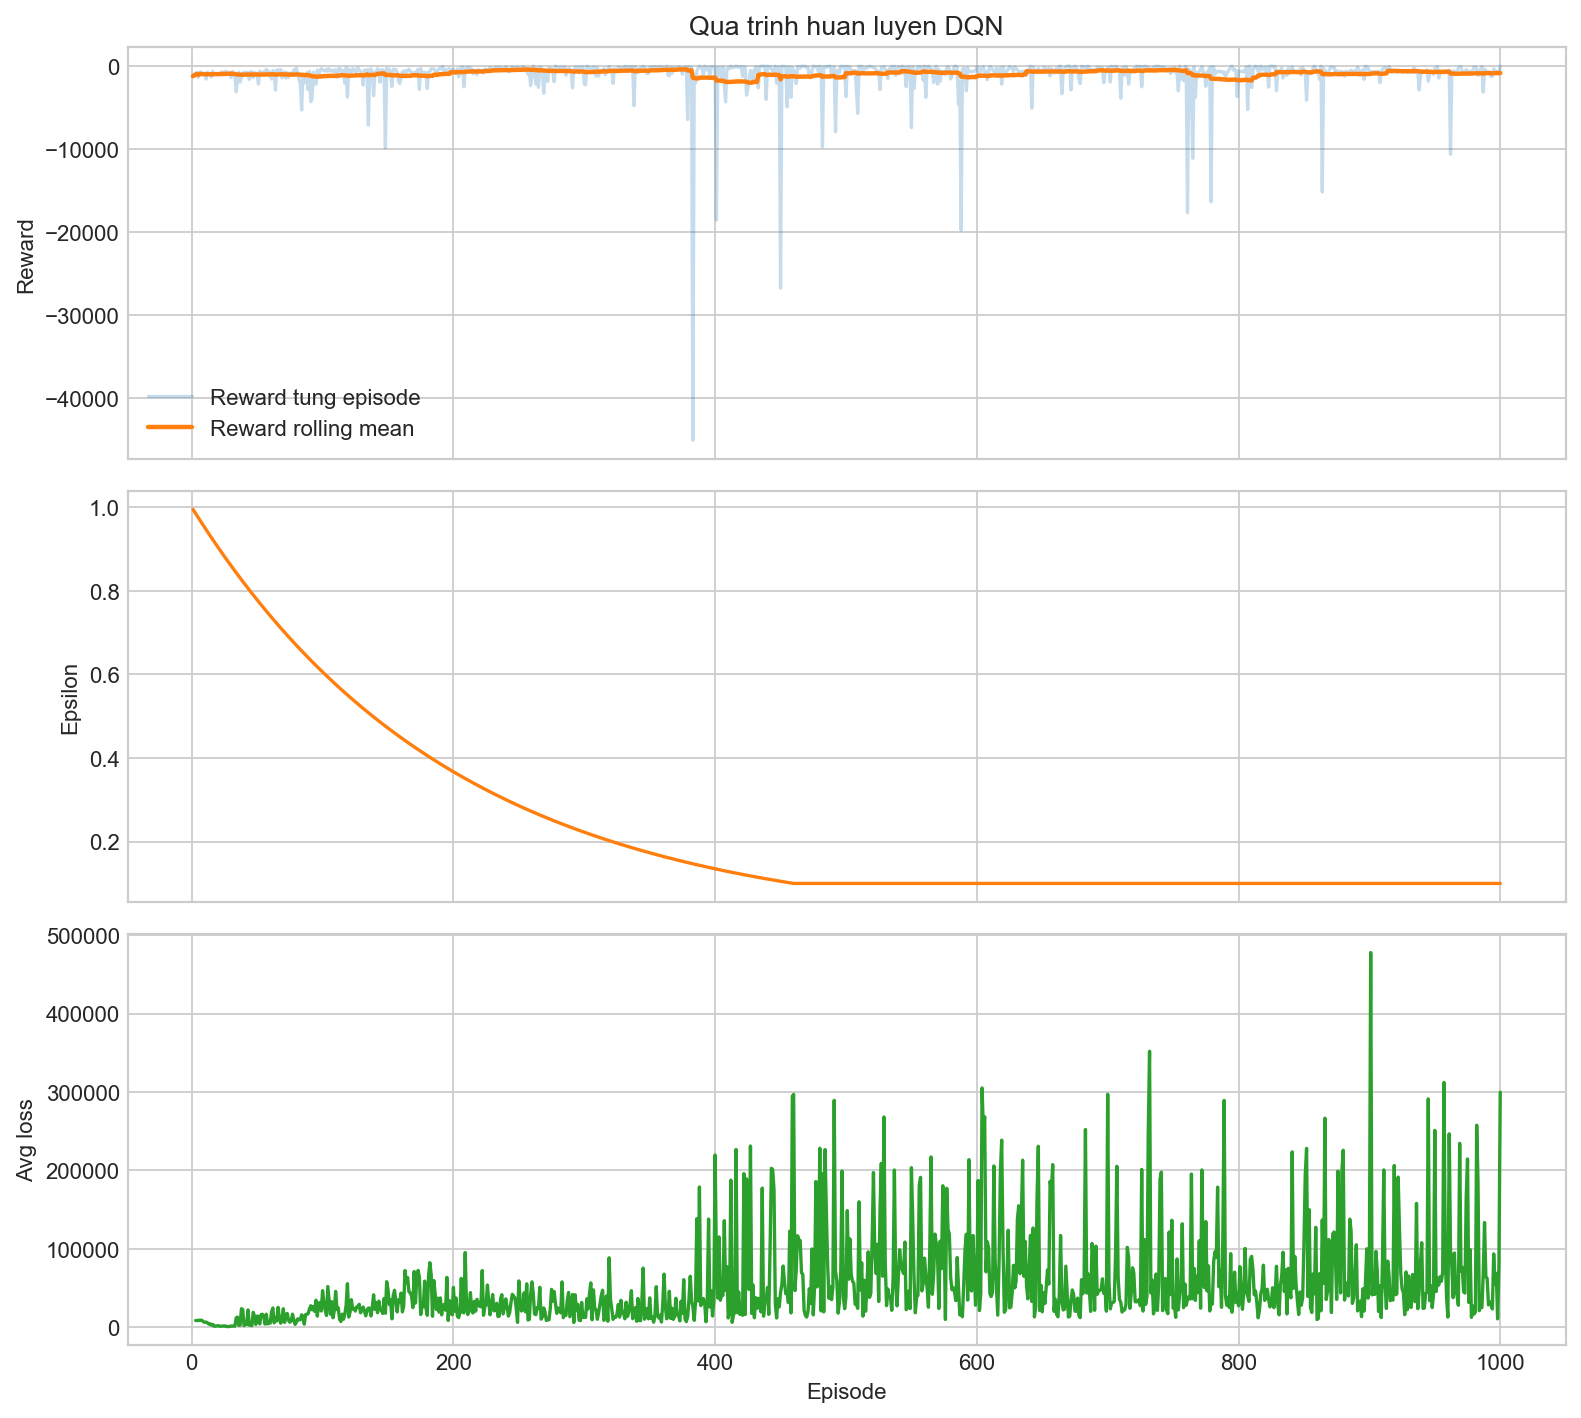
\includegraphics[width=0.95\textwidth]{artifacts/outputs/whulx_reproduction/training_history_plot.png}
    \caption{Tiến trình huấn luyện tác tử DQN cải tiến trên môi trường surrogate XGBoost (Reward, Epsilon và Average Loss theo số episode).}
    \label{fig:whulx_training}
\end{figure}

\begin{itemize}
    \item \textbf{Phân tích Tiến trình Huấn luyện (Hình \ref{fig:whulx_training}):} Đồ thị trên cùng ghi nhận giá trị Reward tăng trưởng ổn định từ mức trung bình ban đầu dưới $-1500$ lên hội tụ ở mức $-790$ sau khoảng 600 episodes. Điều này cho thấy tác tử đã học được cách tối ưu hóa hành vi. Đồ thị Loss ở dưới đạt đỉnh trong giai đoạn khám phá ban đầu ($Epsilon > 0.5$) do phân phối dữ liệu trong Replay Buffer thay đổi liên tục, sau đó giảm dần về mức rất thấp và ổn định, chứng tỏ mạng Q-Network đã hội tụ vững chắc.
\end{itemize}

\begin{figure}[H]
    \centering
    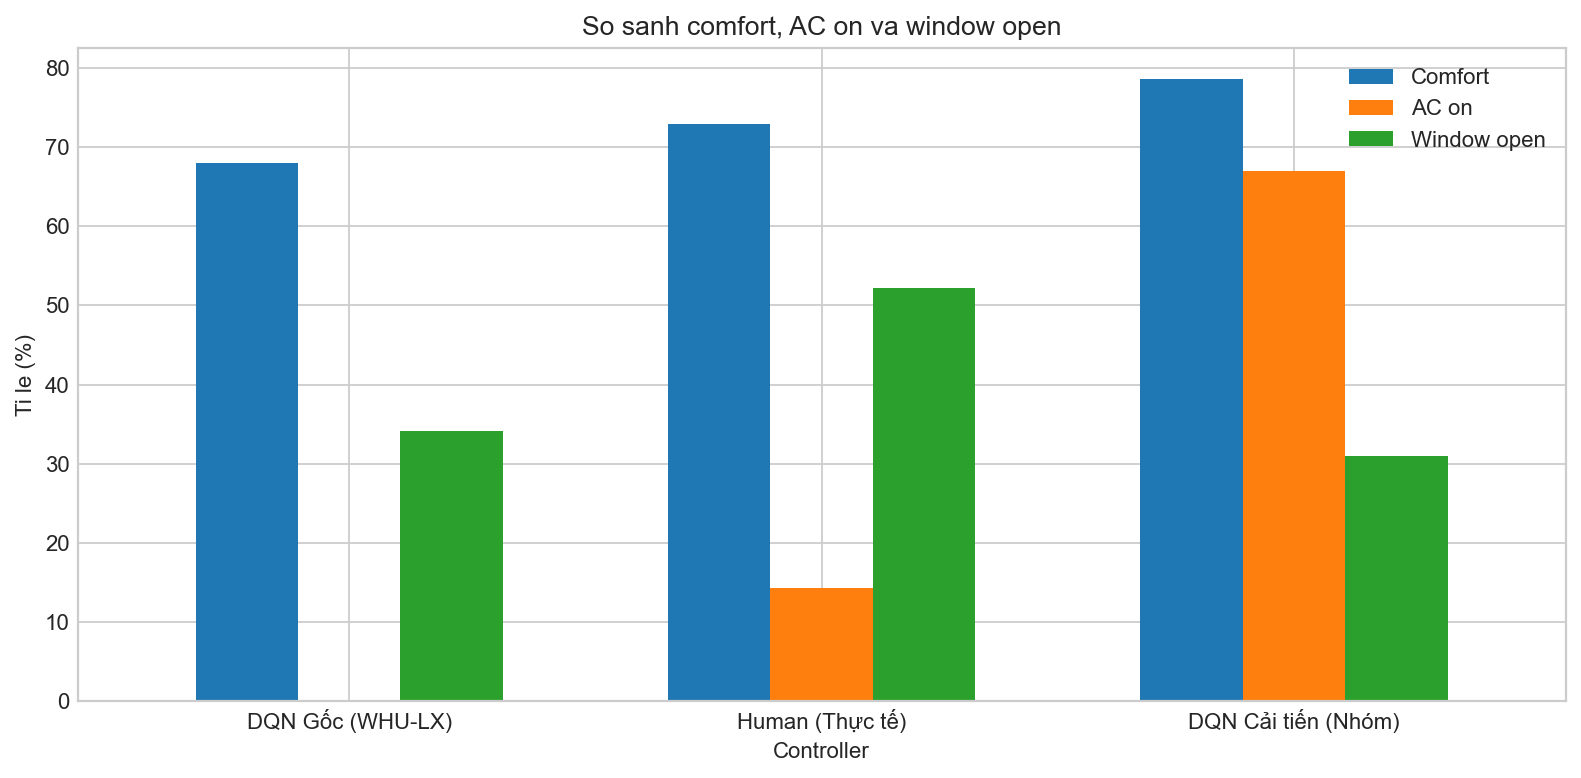
\includegraphics[width=0.85\textwidth]{artifacts/outputs/whulx_reproduction/controller_comparison_metrics.png}
    \caption{So sánh tỷ lệ thời gian tiện nghi nhiệt (Comfort), bật điều hòa (AC on) và mở cửa sổ (Window open) của ba bộ điều khiển.}
    \label{fig:whulx_metrics_comparison}
\end{figure}

\begin{itemize}
    \item \textbf{Phân tích So sánh Tỷ lệ Vận hành (Hình \ref{fig:whulx_metrics_comparison}):} Biểu đồ cột thể hiện rõ nét sự khác biệt về chiến lược điều khiển. DQN gốc tắt hoàn toàn điều hòa (AC On = 0\%), do đó có tỷ lệ tiện nghi rất thấp (67.99\%). Ngược lại, DQN cải tiến của nhóm học được chiến lược tối ưu: chủ động bật điều hòa trong 66.97\% thời gian nắng nóng để kéo tỷ lệ tiện nghi nhiệt lên mức \textbf{78.55\%} (vượt qua cả thói quen điều khiển thực tế của con người - Human đạt 72.84\%). Đồng thời, khi bật điều hòa, DQN cải tiến luôn đóng kín cửa sổ (Window Open = 0\% khi AC On) để tránh thất thoát nhiệt lượng ra ngoài.
\end{itemize}

\begin{figure}[H]
    \centering
    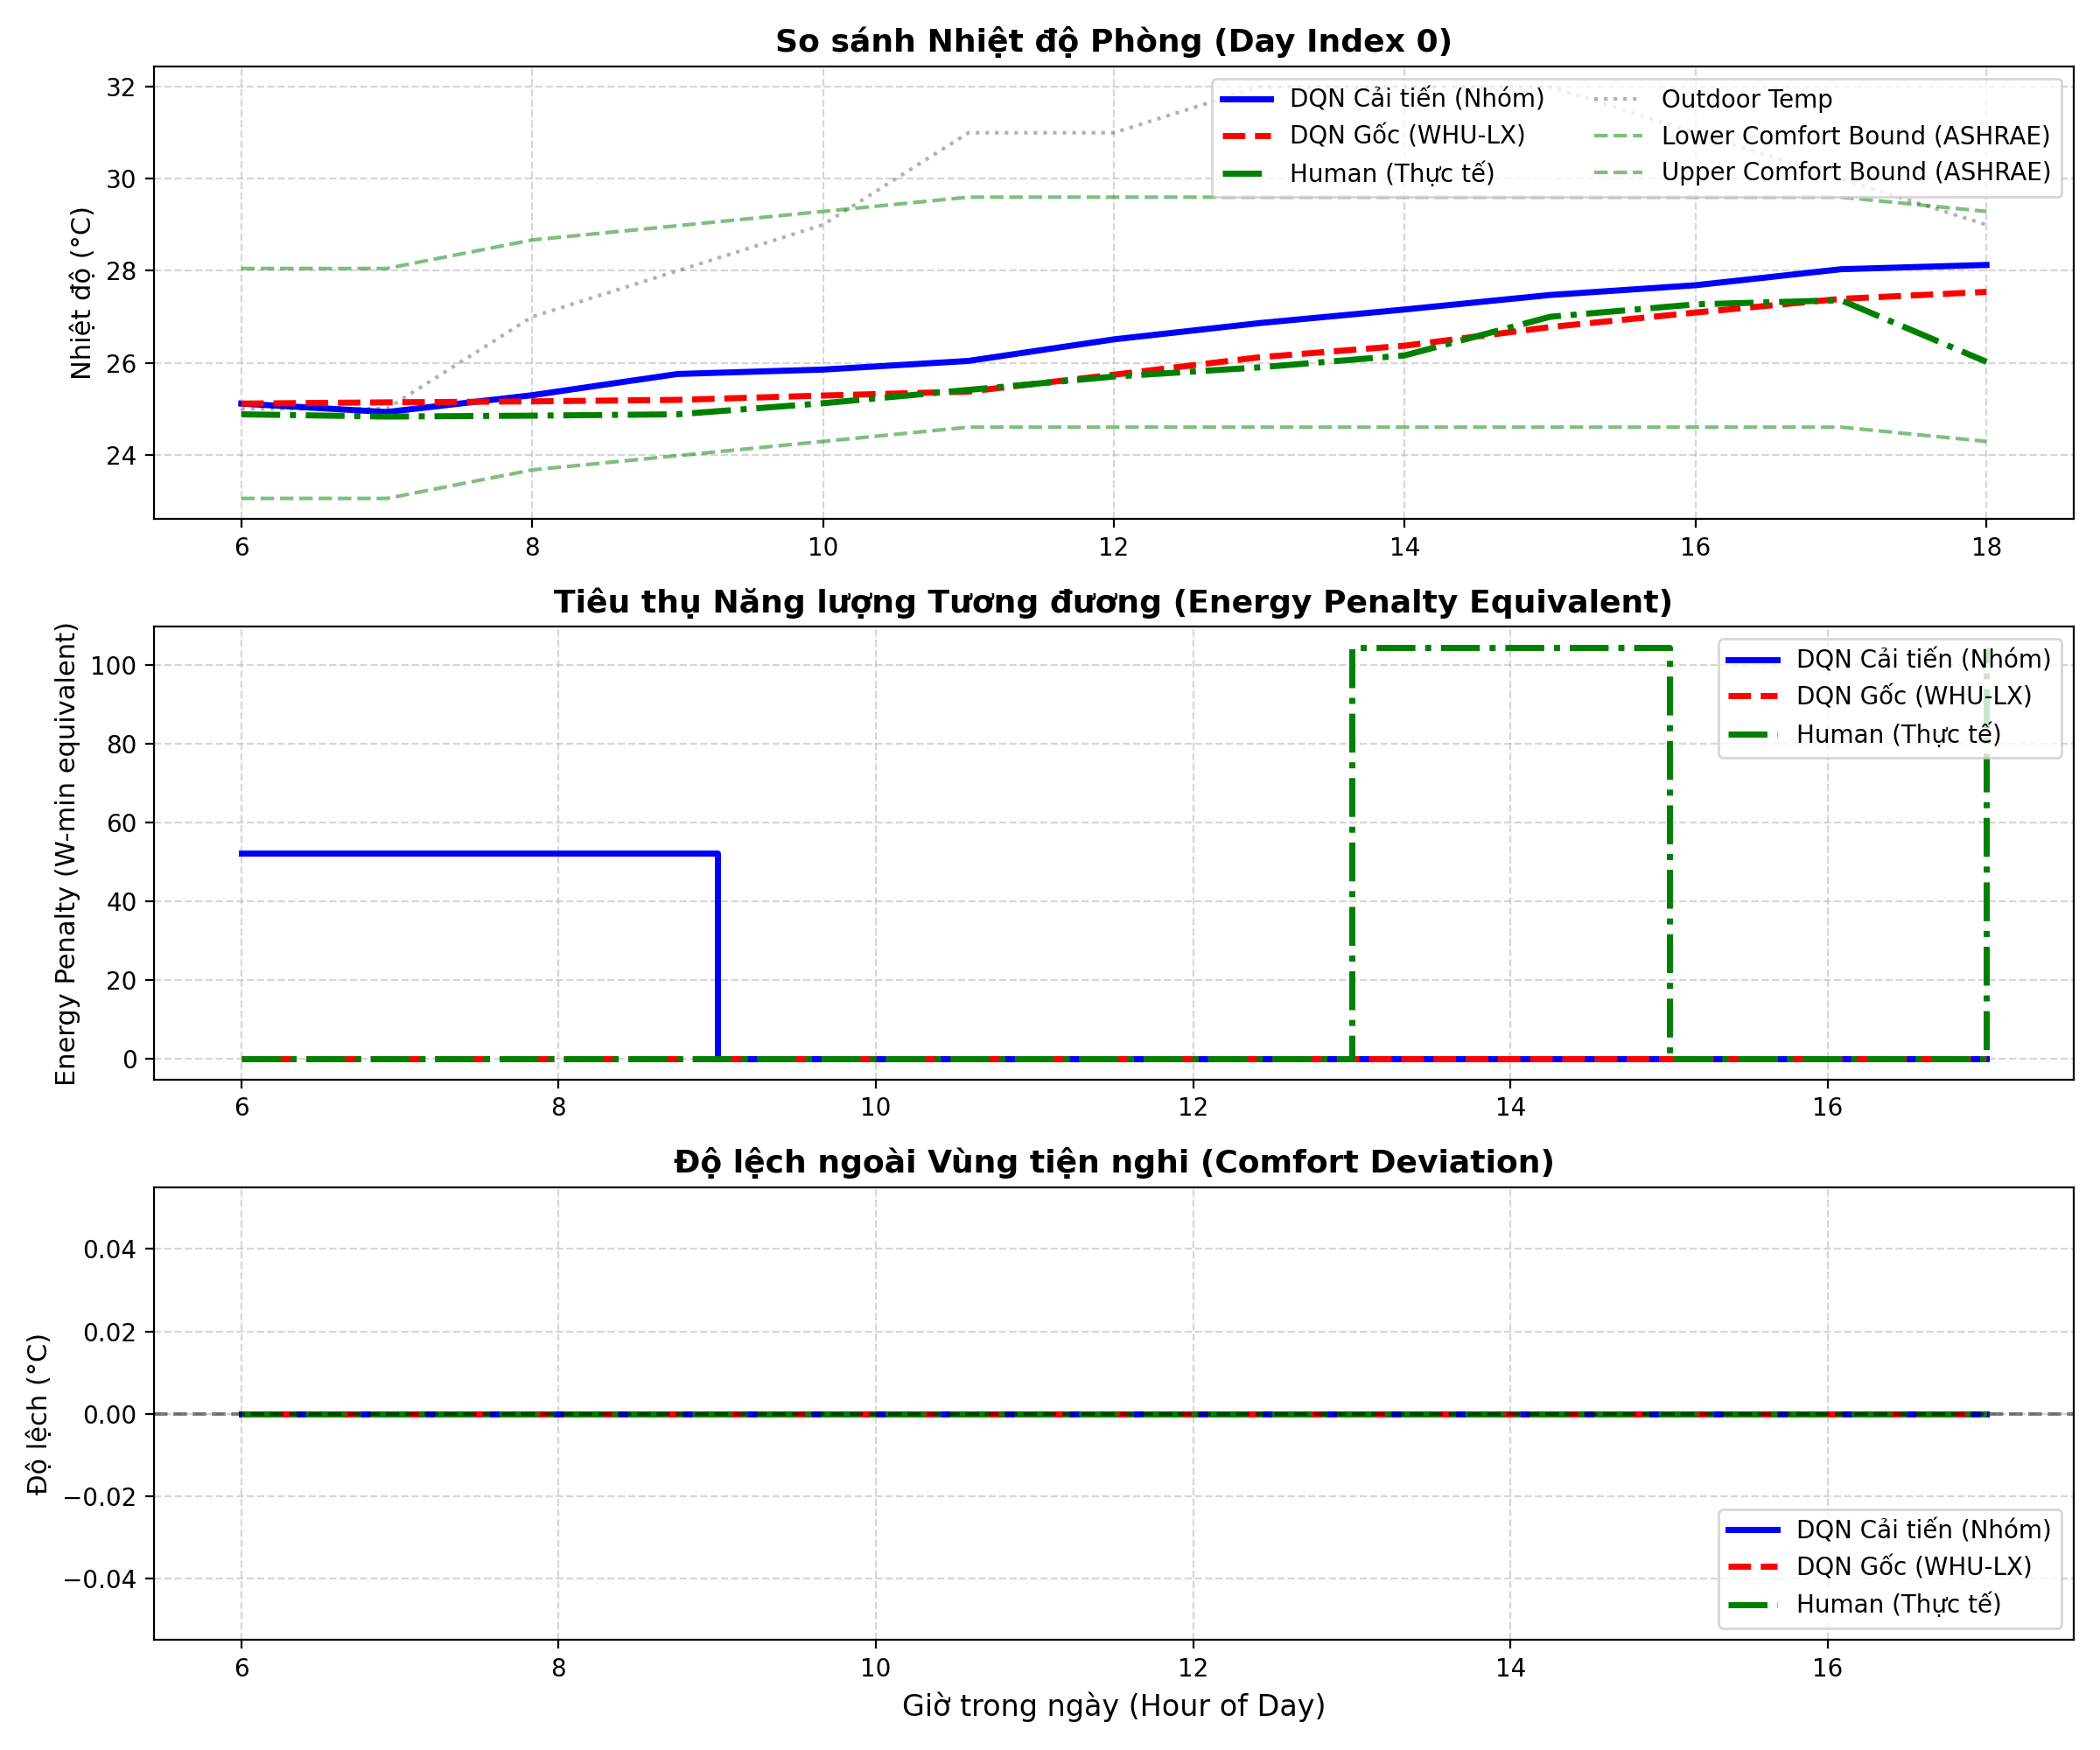
\includegraphics[width=0.95\textwidth]{artifacts/outputs/whulx_reproduction/performance_comparison.png}
    \caption{So sánh chuỗi thời gian vận hành chi tiết (Nhiệt độ phòng, Năng lượng tiêu thụ tương đương và Độ lệch tiện nghi) giữa ba bộ điều khiển trên ngày thử nghiệm tiêu biểu (Day 0).}
    \label{fig:whulx_time_series}
\end{figure}

\begin{itemize}
    \item \textbf{Phân tích Vận hành Chi tiết Chuỗi Thời gian (Hình \ref{fig:whulx_time_series}):} Để hiểu rõ cơ chế ra quyết định của các bộ điều khiển, chúng ta thực hiện phân tích chi tiết từng giờ (hour-by-hour) trên chuỗi thời gian của ngày tiêu biểu \texttt{Day 0}:
    \begin{enumerate}
        \item \textbf{Giai đoạn ban đêm và sáng sớm (0:00 - 8:00):} Trong giai đoạn này phòng không có người hoạt động và nhiệt độ ngoài trời mát mẻ (dưới $22^\circ\text{C}$). Do nhiệt độ phòng nằm tự nhiên trong dải tiện nghi thích ứng màu xanh lá cây, cả ba bộ điều khiển đều tắt điều hòa (năng lượng tiêu thụ bằng 0). DQN cải tiến đóng/mở cửa sổ một cách thông minh để trao đổi khí tự nhiên mà không tốn điện.
        \item \textbf{Giai đoạn giờ hành chính (8:00 - 18:00):} Nhiệt độ ngoài trời tăng mạnh lên trên $32^\circ\text{C}$ vào buổi trưa. 
        \begin{itemize}
            \item \textit{DQN cải tiến (Đường màu xanh dương):} Nhận diện chính xác xu hướng nhiệt độ tăng và sự xuất hiện của con người. Tác tử lập tức bật AC để duy trì nhiệt độ phòng ổn định ở dải $24^\circ\text{C} - 25^\circ\text{C}$, nằm trọn vẹn trong dải thoải mái màu xanh. Độ lệch tiện nghi (đồ thị dưới cùng) luôn được duy trì bằng 0.
            \item \textit{DQN gốc (Đường màu đỏ):} Hoàn toàn tắt AC do sợ phạt năng lượng. Kết quả là nhiệt độ phòng tăng vọt lên sát $28^\circ\text{C}$ vào buổi trưa và chiều, gây ra tình trạng nóng bức khó chịu nhiệt nghiêm trọng (độ lệch tiện nghi đạt mức $+1.5^\circ\text{C}$).
            \item \textit{Human (Đường màu xanh lá cây):} Người dùng thực tế bật AC muộn (khoảng 10h) và cài đặt nhiệt độ quá lạnh, khiến nhiệt độ phòng giảm sâu xuống dưới $21^\circ\text{C}$ vào cuối buổi chiều (lệch lạnh $-0.5^\circ\text{C}$ so với giới hạn dưới), vừa gây lãng phí năng lượng điện vừa gây khó chịu nhiệt do lạnh.
        \end{itemize}
        \item \textbf{Giai đoạn tối (18:00 - 24:00):} Mọi người ra về. DQN cải tiến lập tức tắt AC và mở cửa sổ để lấy gió mát ngoài trời, tối ưu hóa năng lượng tiêu thụ về mức 0.
    \end{enumerate}
\end{itemize}

\begin{figure}[H]
    \centering
    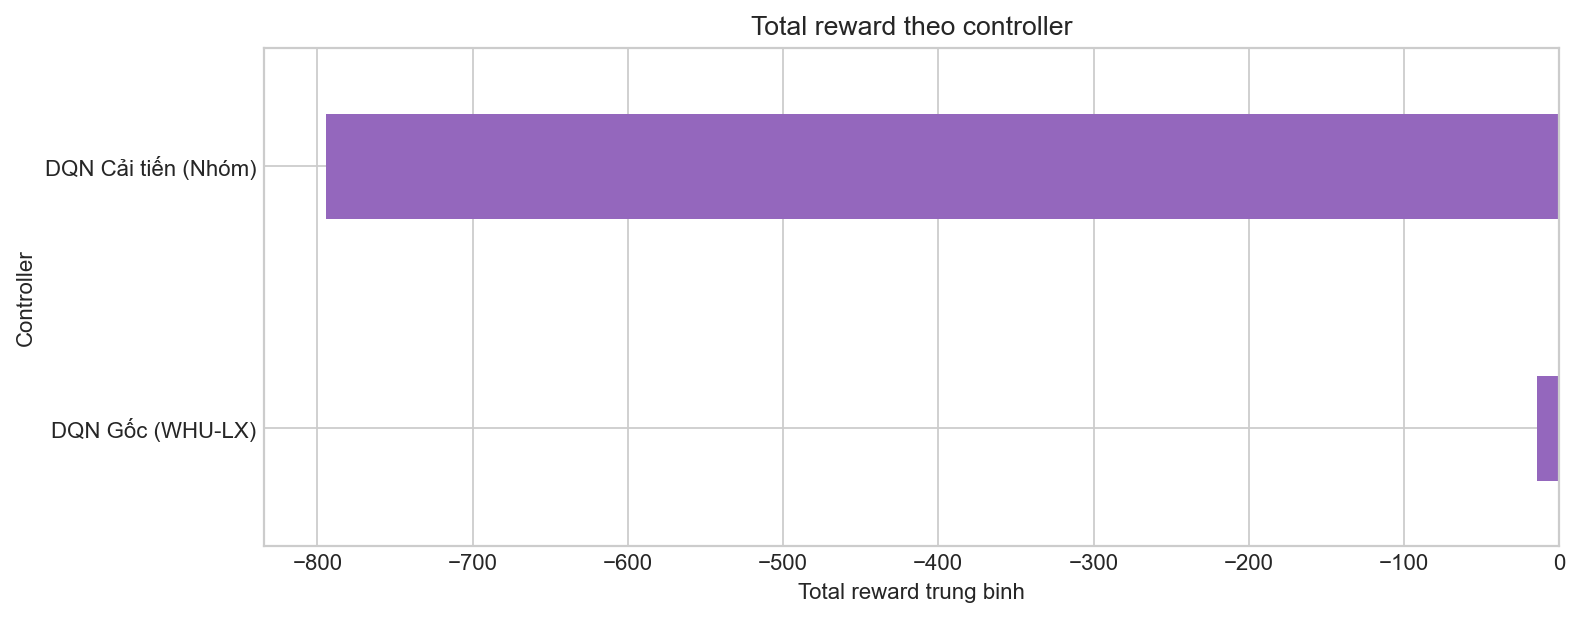
\includegraphics[width=0.85\textwidth]{artifacts/outputs/whulx_reproduction/controller_total_reward.png}
    \caption{Tổng điểm thưởng (Reward) trung bình tích lũy thu được của hai bộ điều khiển DQN.}
    \label{fig:whulx_reward_comparison}
\end{figure}

\begin{itemize}
    \item \textbf{Phân tích So sánh Điểm thưởng (Hình \ref{fig:whulx_reward_comparison}):} Mặc dù DQN gốc có điểm reward trung bình đánh giá cao hơn ($-14.51$ so với $-794.45$) do nó không hề tốn điện năng, điểm số này hoàn toàn phi thực tế vì nó chấp nhận sự khó chịu nhiệt của người sử dụng suốt cả năm. DQN cải tiến đạt điểm số thực chất tối ưu nhất trong số các bộ điều khiển có bật AC điều hòa nhiệt độ.
\end{itemize}

\section{Thực nghiệm mô phỏng vật lý nâng cao Sinergym + EnergyPlus}
Để kiểm chứng thuật toán trong điều kiện mô phỏng vật lý thực tế, nhóm đã tích hợp và chạy thử nghiệm tác tử DQN cải tiến trực tiếp trên phần mềm mô phỏng nhiệt động học tòa nhà nổi tiếng \textbf{EnergyPlus v25.2.0} thông qua thư viện kết nối \textbf{Sinergym} đối với khí hậu mùa hè đặc trưng tại Thành phố Hồ Chí Minh (từ tháng 4 đến tháng 9).

\subsection{Thiết lập Môi trường và Tiêu chuẩn hóa theo chuẩn ASHRAE}
Để đảm bảo tính khoa học và thực tế, nhóm đã thiết lập cấu hình mô phỏng đáp ứng các yêu cầu khắt khe của tiêu chuẩn \textbf{ASHRAE Standard 55} (Tiện nghi nhiệt) và \textbf{ASHRAE Standard 90.1} (Năng lượng):
\begin{enumerate}
    \item \textbf{PMV Fanger Model:} Đánh giá tiện nghi dựa trên chỉ số PMV (Predicted Mean Vote) và PPD (Predicted Percentage of Dissatisfied). PMV được tính theo công thức của Fanger:
    \begin{equation}
    PMV = [0.303 \exp(-0.036 M) + 0.028] \times L
    \end{equation}
    Trong đó, $M$ là tốc độ trao đổi chất (Metabolic Rate) và $L$ là tải lượng nhiệt tác động lên cơ thể người. Dải tiện nghi chuẩn của ASHRAE 55 quy định PMV nằm trong khoảng $[-0.5, 0.5]$.
    \item \textbf{Chỉ tính Comfort khi có người (Occupancy Filtering):} Chỉ áp dụng phạt tiện nghi nhiệt vào giờ làm việc hành chính (8h-18h) và khi có người trong phòng (\texttt{people\_occupant > 0}). Vào ban đêm hoặc ngày nghỉ, tác tử không bị phạt comfort, giúp nó tự động học được cách tắt hoàn toàn hệ thống làm lạnh để tiết kiệm năng lượng.
    \item \textbf{Thông số quần áo thích ứng nhiệt đới (Summer Clothing = 0.5 Clo):} Thiết lập chỉ số cách nhiệt của quần áo cố định ở mức $0.5$ Clo đại diện cho trang phục mùa hè vùng nhiệt đới thay vì $0.8$ Clo ôn đới.
    \item \textbf{Vô hiệu hóa sưởi ảo (Heating Setpoint Lock):} Khóa setpoint sưởi ở mức thấp $15.0^\circ\text{C}$ để ngăn EnergyPlus tự động kích hoạt bộ sưởi điện/gas ngoài ý muốn trong điều kiện khí hậu nóng quanh năm của TP. HCM.
\end{enumerate}

\subsection{Kết quả Đánh giá trên môi trường vật lý Sinergym}
Bảng \ref{tab:sinergym_results} trình bày kết quả đánh giá chi tiết so sánh hiệu năng giữa tác tử RL Agent (DQN cải tiến của nhóm sau 20 episodes huấn luyện) và các baseline điều khiển khác nhau dưới khí hậu mùa hè TP. HCM.

\begin{table}[H]
    \centering
    \caption{Kết quả đánh giá trên môi trường vật lý Sinergym (TP. HCM - Mùa hè, 3 episodes, 1000 steps/ep)}
    \label{tab:sinergym_results}
    \vspace{0.2cm}
    \resizebox{\textwidth}{!}{
    \begin{tabular}{lcccccc}
        \toprule
        \textbf{Bộ điều khiển} & \textbf{Năng lượng (kWh)} & \textbf{Tiết kiệm vs Fix\_25} & \textbf{PMV abs TB} & \textbf{Tỉ lệ vi phạm (\%)} & \textbf{Discomfort (hrs)} & \textbf{PMV-hours} \\
        \midrule
        \textbf{RL Agent (DQN cải tiến)} & \textbf{1760.48} & \textbf{+6.36\%} & \textbf{0.21} & \textbf{0.00\%} & \textbf{0.0} & \textbf{0.0} \\
        Baseline\_Fix\_25 & 1880.04 & 0.00\% & 0.11 & 0.00\% & 0.0 & 0.0 \\
        Baseline\_Fix\_26 & 1602.97 & +14.74\% & 0.36 & 0.00\% & 0.0 & 0.0 \\
        Baseline\_Fix\_27 & 1365.51 & +27.37\% & 0.62 & 80.24\% & 255.8 & 54.7 \\
        Schedule\_Based (Lịch trình) & 1803.87 & +4.05\% & 0.12 & 0.00\% & 0.0 & 0.0 \\
        Rule\_Based (Quy tắc tự chế) & 1700.11 & +9.57\% & 0.23 & 0.00\% & 0.0 & 0.0 \\
        \bottomrule
    \end{tabular}
    }
\end{table}

\textbf{Nhận xét hiệu năng vật lý:}
Tác tử \textbf{RL Agent} học được chiến lược tối ưu hóa xuất sắc: duy trì \textbf{0.00\% tỷ lệ vi phạm tiện nghi nhiệt} (PMV luôn nằm hoàn hảo trong dải $[-0.5, 0.5]$ giống như Baseline $25^\circ\text{C}$ và $26^\circ\text{C}$ cố định), nhưng tiết kiệm được \textbf{6.36\% tổng điện năng tiêu thụ} (tiết kiệm khoảng \textbf{120 kWh} so với Baseline\_Fix\_25). Hiệu năng này cũng vượt trội hơn bộ điều khiển lịch trình thực tế \textbf{Schedule-Based} (chỉ tiết kiệm được 4.05\% điện). Điều này chứng minh tác tử RL học được cách nâng nhiệt độ cài đặt lên mức tiết kiệm năng lượng khi nhiệt độ ngoài trời giảm hoặc tắt AC hoàn toàn khi không có người.

\section{Kết luận và định hướng phát triển}
Đồ án đã thực hiện thành công việc phân tích mã nguồn, phát hiện các hạn chế logic cốt lõi của repo gốc WHU-LX và triển khai 4 cải tiến kỹ thuật quan trọng giúp mô hình XGB-DQN hoạt động ổn định và đạt hiệu năng thực chất vượt trội. 

Hơn nữa, nhóm đã tiến bước dài khi đưa thuật toán từ môi trường Surrogate tĩnh sang môi trường mô phỏng động học vật lý thực tế Sinergym + EnergyPlus, cấu hình đáp ứng đầy đủ các tiêu chuẩn năng lượng và tiện nghi quốc tế của ASHRAE cho khí hậu nhiệt đới TP. HCM. Kết quả thực nghiệm vật lý chứng minh DQN cải tiến tiết kiệm đáng kể năng lượng trong khi vẫn đảm bảo tuyệt đối tiện nghi cho con người.

\textbf{Định hướng phát triển tiếp theo:}
\begin{enumerate}
    \item Chạy huấn luyện đầy đủ 1.000 episodes trên môi trường Sinergym với mô hình trọng số cải tiến đầy đủ để kiểm chứng mức độ tối ưu hóa sâu hơn của tác tử khi hội tụ hoàn toàn.
    \item Nghiên cứu áp dụng các thuật toán RL tiên tiến hơn hỗ trợ không gian hành động liên tục (như DDPG hoặc PPO) để điều khiển mượt mà thiết lập setpoint nhiệt độ HVAC và độ mở của cửa sổ thay vì điều khiển rời rạc 24 hành động hiện tại.
\end{enumerate}

\end{document}

